%\part{Aspectos Gerais}

\chapter[Referencial Teórico]{Referencial teórico}
	
	Este capítulo tem como objetivo servir como referencial teórico para todo o documento. As idéias discutidas neste capítulo são
	
\section{Qualidade}
	O principal produto da engenharia de software é o software, contudo o que tem se vivenciado na realidade brasileira de computação é que o software que está sendo entregue é um software precário e de baixa qualidade. Por ser uma palavra abstrata, o conceito de qualidade é bem amplo, porém o termo qualidade normalmente está associado a uma medida relativa, essa qualidade pode ser entendida como "conformidade às especificações". Conceituando dessa forma, a não conformidade às especificação é igual a ausência de qualidade \cite{Paduelli}.
\\ A ISO 9126-1 proposta em 2001, também conhecida como Engenharia de Software - Qualidade do Produto, descreve o modelo de qualidade voltado para o produto de software como sendo composto por duas categorias como pode ser visto na Figura \ref{img:relacao_iso}. A primeira categoria está relacionada a qualidade interna e a qualidade externa do software. A segunda categoria se relaciona com a qualidade de uso do software \cite{_nbr_2016}
\graphicspath{{figuras/}}
\begin{figure}
\centering
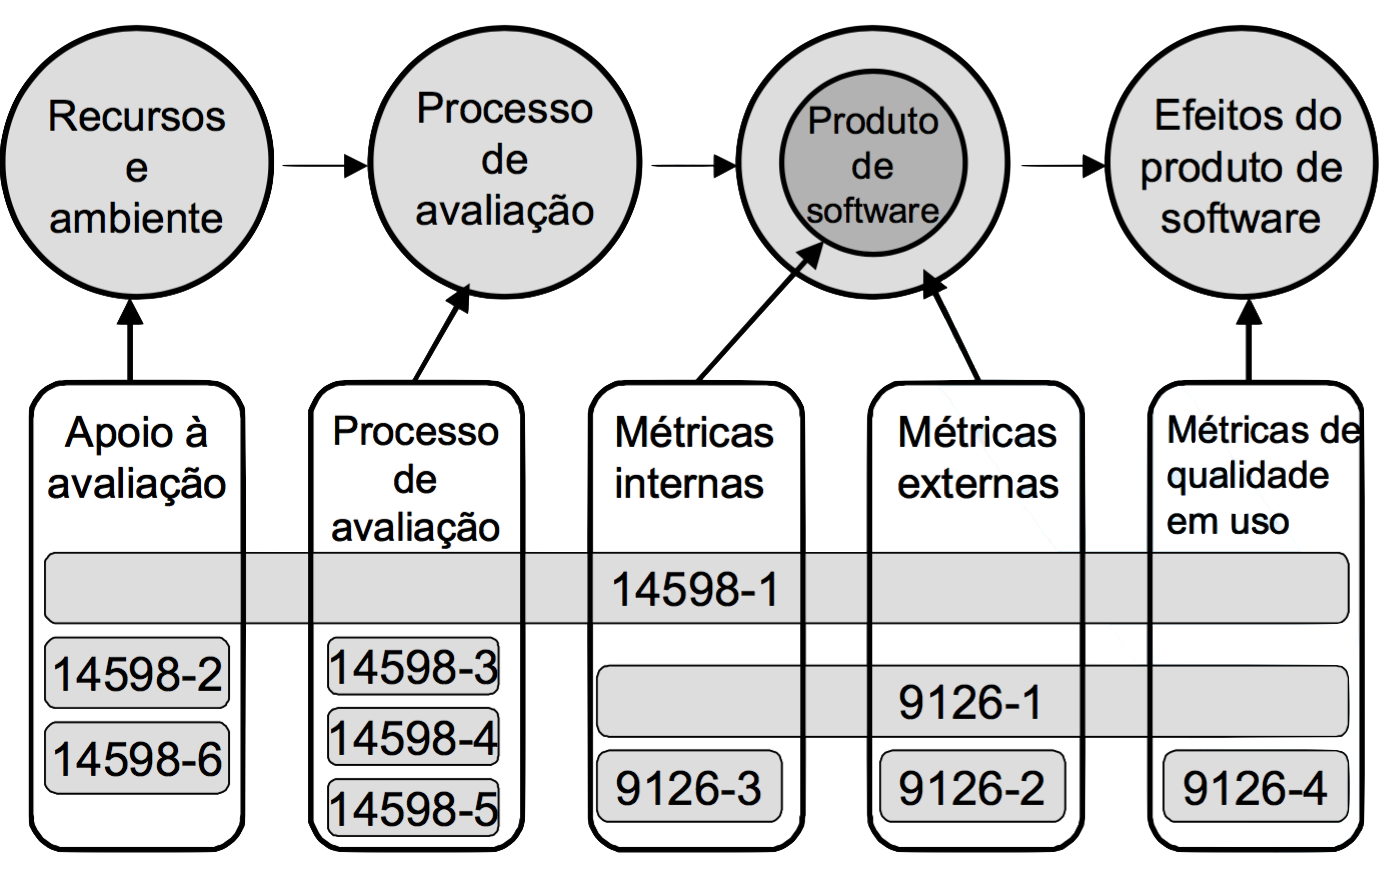
\includegraphics[scale=0.40]{ISO}
\caption{Relação entre as NBR ISO/IEC 9126 e NBR ISO/IEC 14598 .Fonte:\cite{_nbr_2016}}
\label{img:relacao_iso}
\end{figure}
\\ Sob o aspecto de modelo de qualidade,a ISO 9126 classifica a qualidade interna do produto como sendo o somatório das características do ponto de vista interno do software. Os principais produtos desta categoria são os de cunho intermediário, entre eles: relatórios de analise estática do código fonte, revisão dos documentos produzidos, entre outros. A qualidade externa por sua vez já apresenta o seu foco mais voltado para as relações externas do software, normalmente esta relacionado com a execução do código coletando suas métricas enquanto o software está em funcionamento. A Figura \ref{img:modelo_qualidade} apresenta a divisão proposta pela \cite{_nbr_2016} onde são categorizados seis aspectos de qualidade de software e suas subcaracterísticas, essas podem ser medidas por meio de métricas internas e externas. 
 \graphicspath{{figuras/}}
\begin{figure}
\centering
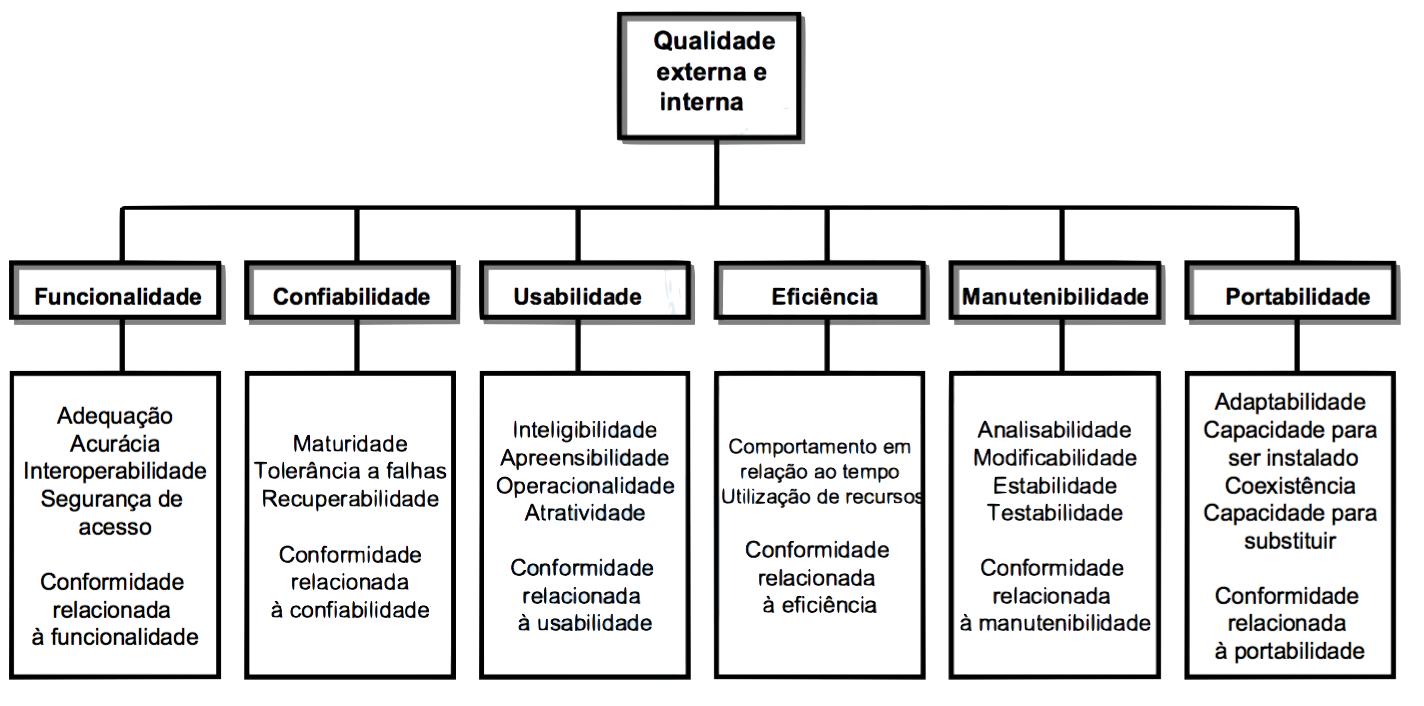
\includegraphics[scale=0.50]{Modelo_de_Qualidade}
\caption{Modelo de Qualidade para Qualidade Interna e Externa .Fonte:\cite{_nbr_2016}}
\label{img:modelo_qualidade}
\end{figure}
\\Segundo a ISO 9126 essas caracteristicas podem ser definidas como:
\begin{itemize}
\item \textbf{Funcionalidade}: Capacidade do produto de software de prover funções que atendam às necessidades explícitas e implícitas, quando o software estiver sendo utilizado sob condições especificadas.
\item \textbf{Confiabilidade}:Capacidade do produto de software de manter um nível de desempenho especificado, quando usado em condições especificadas.
\item \textbf{Usabilidade}: Capacidade do produto de software de ser compreendido, aprendido, operado e atraente ao usuário, quando usado sob condições especificadas.
\item \textbf{Eficiência}: Capacidade do produto de software de apresentar desempenho apropriado, relativo à quantidade de recursos usados, sob condições especificadas.
\item \textbf{Manutenibilidade}: Capacidade do produto de software de ser modificado. As modificações podem incluir correções, melhorias ou adaptações do software devido a mudanças no ambiente e nos seus requisitos ou especificações funcionais.
\item \textbf{Portabilidade}: Capacidade do produto de software de ser transferido de um ambiente para outro.
\end{itemize}
Em 2011 surgiu um conjunto de normas conhecidos como SQuaRE que traziam um framework aprimorado à atual norma vigente. Este framework tinha como objetivo avaliar o produto de qualidade de software.

\subsection{Normas SQuaRE}
Este conjunto de normas surgiu para substituir a ISO/IEC 9126, Engenharia de Software - Qualidade do Produto. ISO/IEC 25010 mantém as características de qualidade com alguns incrementos.

\begin{itemize}
\item O escopo dos modelos de qualidade foram extendidos para incluir sistemas computacionais e a qualidade em uso pelo ponto de vista do sistema
\item Segurança foi adicionada como característica, e não uma subcaracterística de funcionalidade.
\item Compatibilidade foi adicionada como característica.
\item A qualidade interna e externa foram combinadas como modelo de qualidade de produto.
\end{itemize}

A norma apresenta três guias de qualidade. O primeiro modelo é referente à Qualidade do Produto, o segundo da Qualidade em Uso e o último Qualidade de Dados.O modelo de Qualidade do Produto subdivide um sistema de software em oito categorias como mostra a imagem \ref{img:modelo_square}.
\graphicspath{{figuras/}}
\begin{figure}
\centering
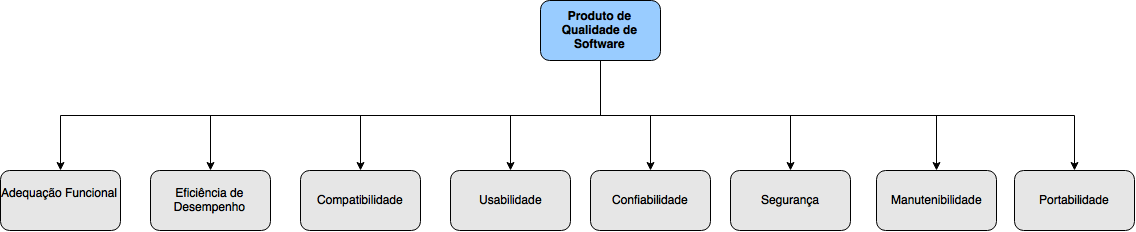
\includegraphics[scale=0.40]{SQuaRE}
\caption{Produto de Qualidade de Software.Fonte:\cite{Square}}
\label{img:modelo_square}
\end{figure}

Este trabalho tem seu desenvolvimento focado no modelo de Qualidade de Uso que apresenta características externas ao software \cite{Square}. O foco deste trabalho está em medir indicadores quanto à manutenção do software.  

\subsection{Manutenção de Software}
Segundo Sommervile \cite{sommervile} manutenção de software é o processo de alterar o sistema depois que ele foi alterado. As alterações feitas no software podem ser simples correções de erro, a até mudanças significativamente grandes que corrigem falhas arquiteturais, ou mesmo melhorias para acomodar novos requisitos.
\\Outra visão sobre manutenção de software é dada por Pressman \cite{pressman} em que o autor conceitua o termo como sendo a correção de defeitos, adaptação do software para atender uma mudança do ambiente e aperfeiçoar as funcionalidades para que atendam às necessidades dos usuários. Outra característica do processo de manutenção é a sua composição por um conjunto de sub processos, atividades e tarefas que podem ser utilizados durante a fase de manutenção para alterar um produto de software, contanto que seja mantido o seu funcionamento \cite{calazans_avaliacao_2005}.
\\Para Sommervile existem quatro categorias de manutenção:
\begin{itemize}
\item \textbf{Manutenção Corretiva}: seu objetivo está em identificar e remover falhas de software
\item \textbf{Manutenção Adaptativa}: provê modificações no software para alojar mudanças no ambiente externo. Nesta manutenção também está incluso o processo de migração para diferentes plataformas tanto de software quanto de hardware.
\item \textbf{Manutenção Perfectiva}: está manutenção é feito com o intuito de aperfeiçoar o software, além dos requisitos funcionais originais. Esta expansão dos requisitos traz consigo uma melhoria às funcionalidades até então implementadas ou um ganho de performance do sistema.
\item \textbf{Manutenção Preventiva}: implementada para permitir que seja mais simples a correção, adaptação ou melhoria do software.
\end{itemize}
